\documentclass{article}
\usepackage{amsmath}
\usepackage{amsfonts}
\usepackage{amssymb}
\usepackage{courier}
\usepackage{graphicx}
\usepackage{subfig}
\usepackage{listings}
\usepackage[margin=1in]{geometry}

\title{Visualization of Open Source Projects}
\begin{document}


\begin{titlepage}
    \begin{center}
        \vspace*{2.5cm}
        {\bf Visualization of Open Source Projects}
        
        \vspace{0.5cm}
        
        Analyzing trends in Github Organizations
        
        \vspace{2.0cm}
        
        \begin{figure}[h!]
	  \centering
	  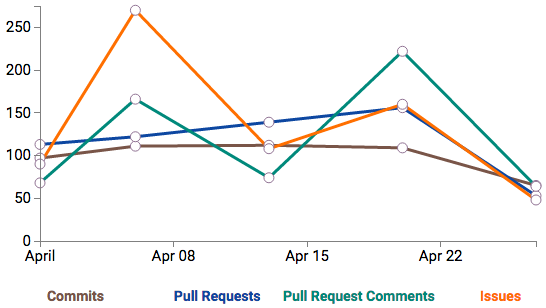
\includegraphics[height=4cm, width=8cm]{cover}
	  \end{figure}

        
        \vspace{2.0cm}        
        
        \hspace{1.5cm} \textbf{David Leonard} \hspace{2.5cm} \textbf{Liron Shimrony}
        
        \vspace{0.5cm}
        \hspace{1.1cm} DrkSephy1025@gmail.com \hspace{1.5cm} lsxliron@gmail.com
	
		\vspace{1.5cm} 
	\textbf{Date}: May 12, 2016
	
	\vspace{1.5cm}
	
	\begin{figure}[b]
          \centering
          \subfloat{{
\includegraphics[width=4cm]{logo2.png} }}
          \qquad
          \subfloat{{
\includegraphics[width=4cm]{logo3.jpg} }}
      \end{figure}
        
        \vspace{1in}
        \vfill
        
    \end{center}
\end{titlepage}

\tableofcontents

\newpage

\section {Introduction}

One of the biggest and most interesting data sources online is \textbf{source code} stored in various version control platforms, such as \textbf{Github} and \textbf{Bitbucket}. These platforms contain various projects stored in \textbf{repositories}, which contain various metadata with which we can draw several conclusions from. This metadata consists of metrics such as:

\begin{itemize}
	\item \textbf{Commits}: Snapshots of the codebase at a given point in time.
	\item \textbf{Issues}: Feature requests and bug reports for a given project.
	\item \textbf{Pull Requests}: Code patches submitted by various other contributors  around the world.
\end{itemize}

The challenge here is to discover various trends in the data with which may not be visible depending on the visualizations chosen to represent the data. However, it is infeasible to analyze every single repository across Github or Bitbucket for this project - as the number of repositories is in the millions. In order to draw meaningful conclusions from the data, we will be selectively analyzing open source projects on Github pertaining to the \textbf{Facebook} organization. The choice for this is arbitrary, but we chose Facebook because it is responsible for open sourcing various projects in the last few years which have heavily influenced the open source community. From this data, we expect to draw various conclusions regarding the lifespan of their open source projects and how they progress over time.

\section {Why?}

Given the general form of the data, the big challenge is to come up with a meaningful visualization which allows us to derive some conclusions.  There have been several projects which strictly visualize \textbf{commits} in a given repository, which typically generate a tree-like structure (or a structure in general). These visualizations show how large a project gets over the course of time as the number of developers and commits increases. While the structures that are generated at the end of these visualizations are interesting to look at, it is difficult to draw any sort of meaningful conclusions. In the next few sections, we briefly show some popular works in this domain.

\subsection {Code Swarm}

Code Swarm [2] is a visualization of commits in a repository, which was also created by Michael Ogawa [1]. Code Swarm represents files as moving elements, where files are mapped to the developer which created it. Moreover, these files are color coded based on whether or not they are source code or general documents. When developers drop off in their contributions, they fade over time from the underlying histogram at the bottom which allows us to keep track of what events have occurred before in the timeline. Code Swarm is able to visualize a wide spectrum of repository types: 

\begin {itemize}
	\item {Subversion}
	\item {CVS}
	\item {Git}
	\item {Mercurial}
	\item {Perforce}
	\item {VSS}
	\item {Starteam}
	\item {Wikiswarm}
	\item {Darcs}
\end {itemize}

\begin{figure}[h!]
\centering
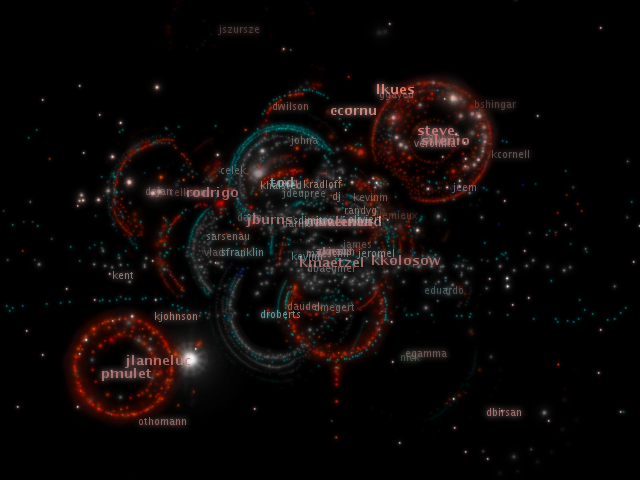
\includegraphics[height=8cm, width=12cm]{swarm}
\caption{Code Swarm}
\end{figure}

\subsection {Gource}

Another popular source code visualization tool is \textbf{Gource}, which also generates a tree-like structure of the repository similar to Code Swarm. Gource is able to visualize \textbf{git}, \textbf{subversion}, \textbf{mercurial} and \textbf{bazaar} repositories. These visualizations consist of the root directory being mapped to the root of the tree, while directories will become branches and subsequent files become leaf nodes as time elapses from the conception of the repository to the last commit. 

\begin{figure}[h!]
\centering
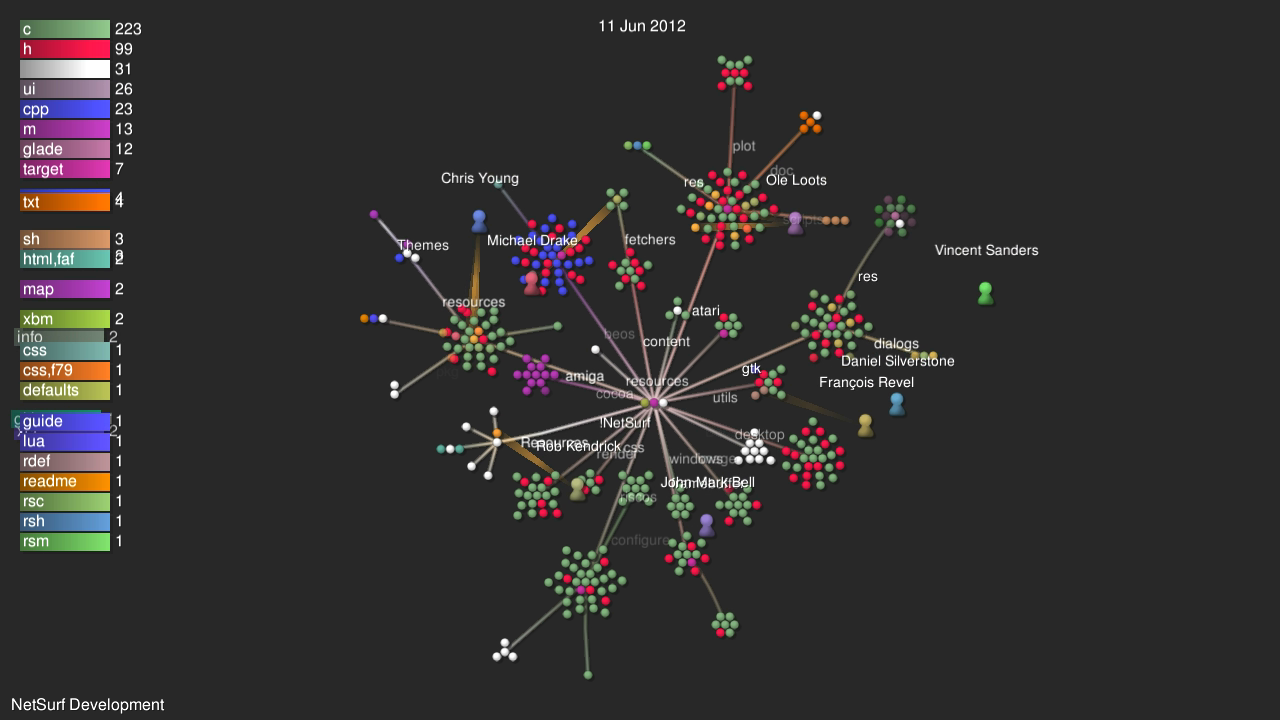
\includegraphics[height=8cm, width=12cm]{gource}
\caption{Gource Visualization}
\end{figure}

\subsection {Github Visualizer}

One of the most comprehensive open source visualization tools is \textbf{Github Visualizer}[4], which was built using d3\footnote{d3: https://d3js.org/} and the Github API\footnote{Github API: https://developer.github.com/v3/}. Using this tool, one may visualize events in a Github repository ranging from commits to lines of code over time. During the runtime of the visualization, a histogram is built along the time-axis showing the density of events for the current time frame. Moreover, a user may choose to visualize an individual repository belonging to a user, or they may visualize all repositories which belong to a given user. By hovering over various elements in the visualization, we can drill down deeper and analyze the lines of code that are added over time per time series event. For reference, we have included a visualization of Facebook repositories generated by this tool in Figure 3.

\begin{figure}[h!]
\centering
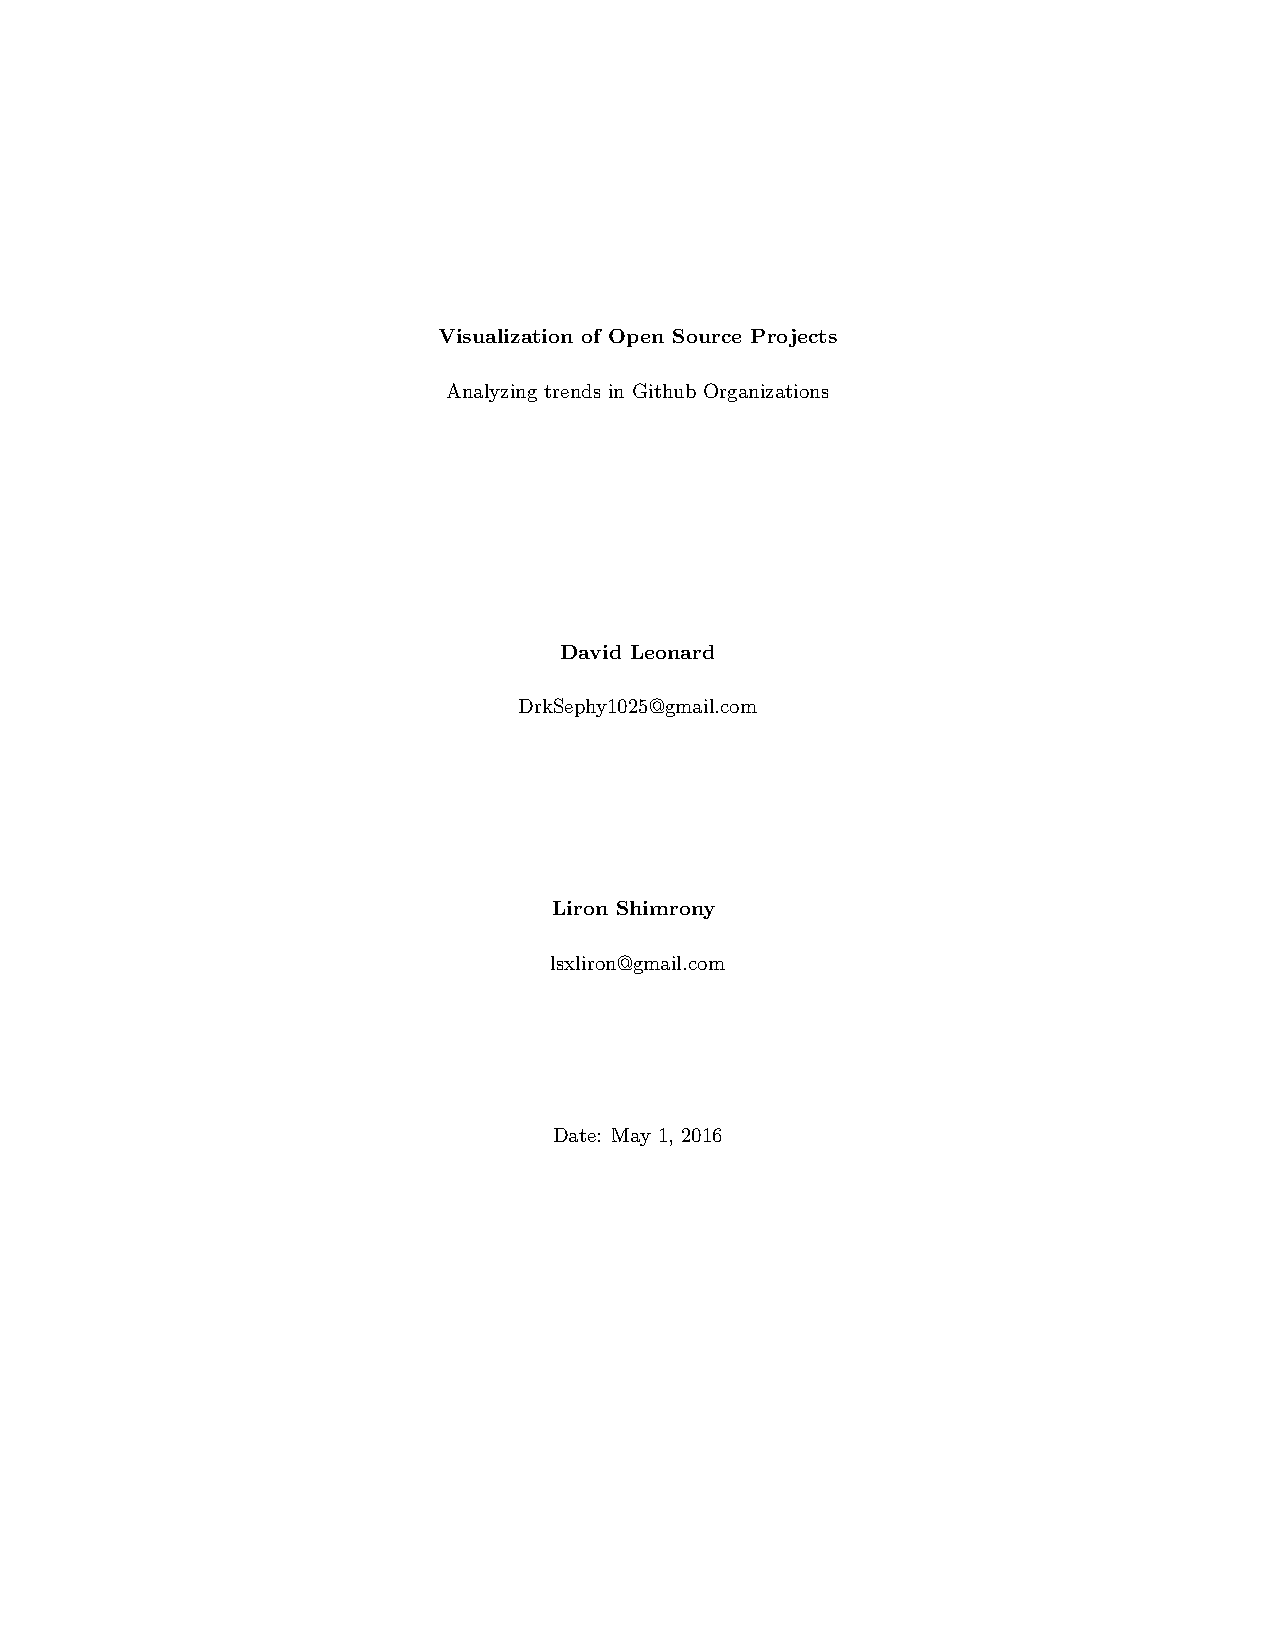
\includegraphics[height=10cm, width=16cm]{viz}
\caption{Github Visualizer: Facebook Repositories}
\end{figure}

While this visualization is very interesting to look at, we fell that it is too dense and it becomes a challenge to narrow down on a particular aspect of the visualization. It is hard to draw any solid conclusions from what is presented, and trends are hard to discover apart from the event density histogram. In our own project, we aim to build a series of visualizations which are simple yet powerful with respect to the trends that can be discovered.

\section {What?}

In this section we discuss the visualizations which we have created over the span of this project. As mentioned earlier, this project was created without knowing the questions we want to answer, but we expect several noticeable trends to crop up throughout the lifespan of the open source projects analyzed. We begin by discussing our first visualization: the \textbf{event bar chart}.

\vspace{1.0cm}

\subsection {Event Bar Chart}

Our first goal was to show the sum totals of various events across all Facebook repositories on Github over a given time frame. These events are:

\begin {itemize}
	\item \textbf{Commit Comments}: The number of comments made on an individual line of code.
	\item \textbf{Forks}: The number of fork events.
	\item \textbf{Stars}: The number of stargazer (star) events.
	\item \textbf{Pull Requests}: The number of pull request events.
	\item \textbf{Issues}: The number of issue events (issue opened, assigned, closed).
	\item \textbf{Issue Comments}: The number of issue comments made.
	\item \textbf{Commits}: The number of commits made.
\end {itemize}

By viewing the raw totals of these numbers, we can get a high level understanding of what types of events are happening and how they correlate to each other. 
For example, repositories such as \textbf{React} may have more issue events then commits, which could correlate to a period of time in which a new patch or version was released.

\begin{figure}[h!]
\centering
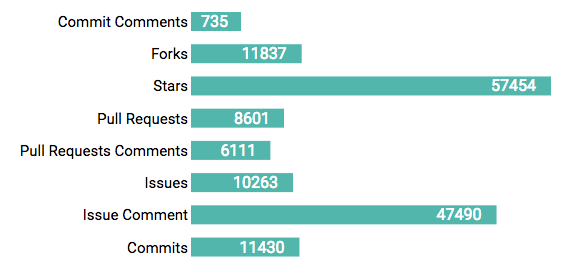
\includegraphics[height=8cm, width=16cm]{bar}
\caption{Events Bar Chart}
\end{figure}

Next we visualized the events over weekly time using a \textbf{Time Series}, which we discuss below.

\subsection {Event Time Series}

Our next train of thought was to create a visualization which demonstrates the change over time of \textbf{Commits}, \textbf{Pull Requests}, \textbf{Pull Request Comments} and \textbf{Issues}. As such, we decided that a time series graph would be perfect for the story we would like to tell. Our reasoning for choosing to visualize these parameters is that they allow us to quickly understand what is going on in a project - a high number of issue events versus low commits correlates to several bugs / feature requests being made. If we factor in the pull requests, a low number versus a high number of issue events means that bugs are being resolved at a small rate. We discuss more of our conclusions in section 5.

\begin{figure}[h!]
\centering
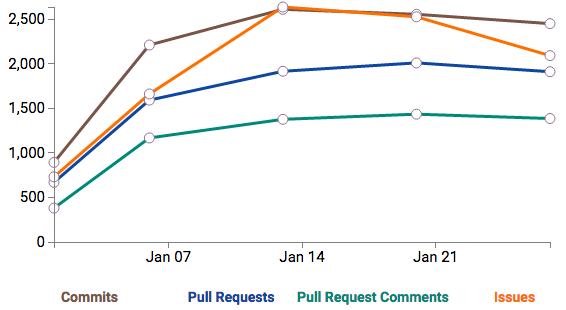
\includegraphics[height=6cm, width=10cm]{time}
\caption{Weekly Event Time Series}
\end{figure}

\subsubsection {Event Time Series Interactivity}

In order to single out particular events and trends, the legend is interactive in that the user can click on any event name to make the corresponding line disappear from the time series. As expected, repeated clicks will toggle the respective lines on and off.

\begin{figure}[h!]
\centering
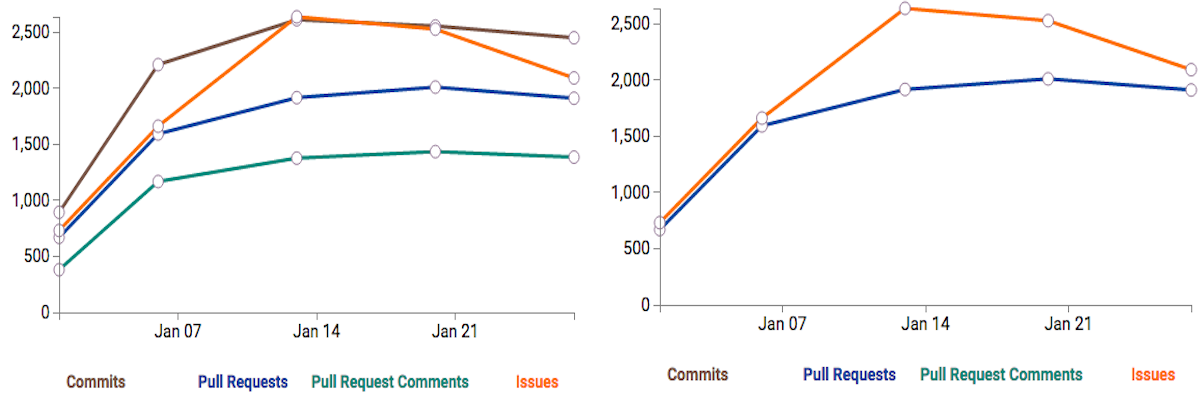
\includegraphics[height=6cm, width=16cm]{combined}
\caption{Interaction with Time Series Legend}
\end{figure}

Lastly, users may hover over any point to view the datapoint in isolation.

\begin{figure}[h!]
\centering
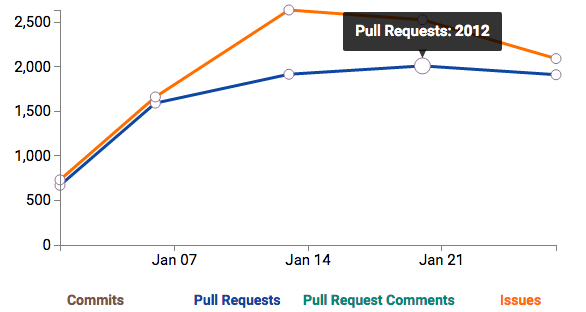
\includegraphics[height=6cm, width=10cm]{hover}
\caption{Time Series Hover Interaction}
\end{figure}

\subsection {Repository Tree Map}

As our visualization stands with the Event Bar Chart and Event Time Series, we currently have no way to drill down and inspect data for individual repositories. As such, as have created a \textbf{Repository Tree Map} which allows the user to specify the repository with which they would like to get detailed data on, as well as a multitude of interactions. On initial page load, the tree map is structured with respect to the number of stars that each repository has.

\begin{figure}[h!]
\centering
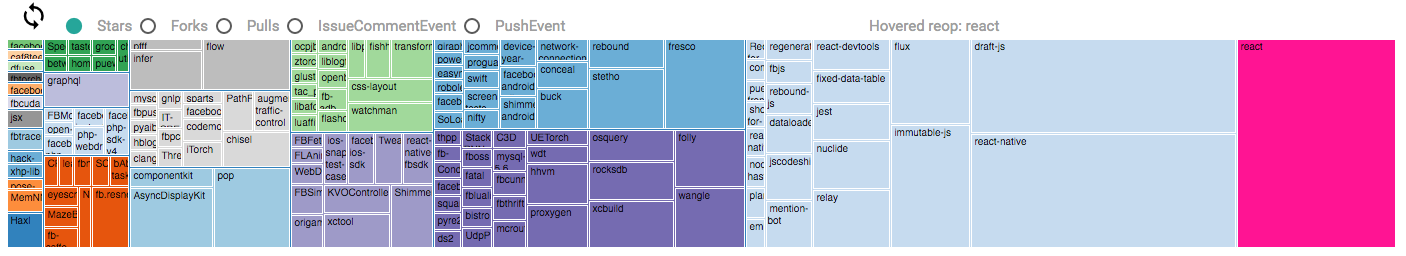
\includegraphics[height=4.5cm, width=17cm]{tree}
\caption{Tree Map Initial Configuration}
\end{figure}

\subsubsection {Repository Tree Map Interactions}

Being the most important visualization of our project, it should have several useful interactions. The first is the ability to see which repository is being hovered over, as indicated by the helper text as well as the color highlighting. The user is also able to rebuild the tree map using the following filters:

\begin {itemize}
	\item \textbf{Stars}: The total number of stars in the given repository.
	\item \textbf{Forks}: The total number of forks in the given repository.
	\item \textbf{Pulls}: The total number of pull requests in the given repository.
	\item \textbf{IssueCommentEvent}: The total number of issue comments in the given repository.
	\item \textbf{PushEvent}: The total number of commits in the given repository.
\end {itemize}

One such example is rebuilding the tree map by the number of issue comments, as shown in Figure 9. It is immediately apparent that the \textbf{react-native} repository has a staggering amount of issue comments, which is due to it's recent popularly and youth. Currently, react-native is 
a bleeding-edge project which allows developers to create mobile applications using JavaScript (and in particular, using \textbf{react}). As such, many bugs are being discovered, as well as features and contributions. Unsurprisingly, react-native is also the leader with respect to pull requests and commits - this being just one of the trends that are easily discovered through the tree map.

\newpage

\begin{figure}[h!]
\centering
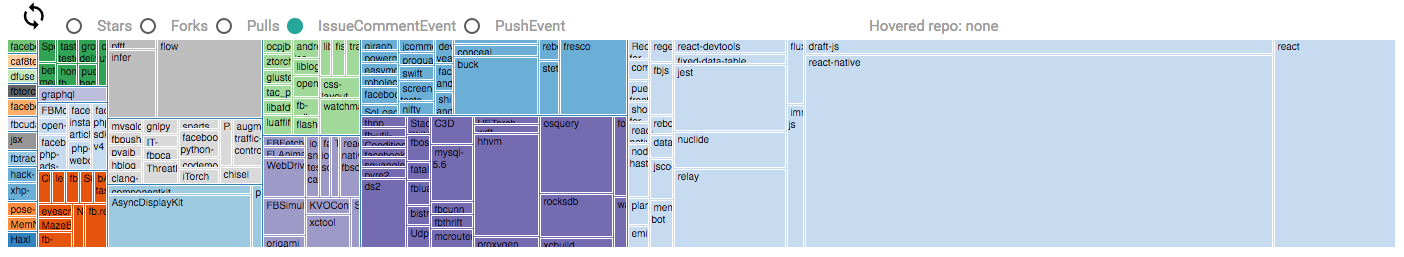
\includegraphics[height=4.5cm, width=17cm]{comment}
\caption{Tree Map structured by Issue Comments}
\end{figure}

\subsubsection {Repository snapshot}

As stated earlier, clicking on any individual repository will allow us to drill down to view metrics specific to that repository. For example, clicking \textbf{react-native} on the tree map will update both the event bar chart and event time series with data specific to react-native:

\begin{figure}[h!]
\centering
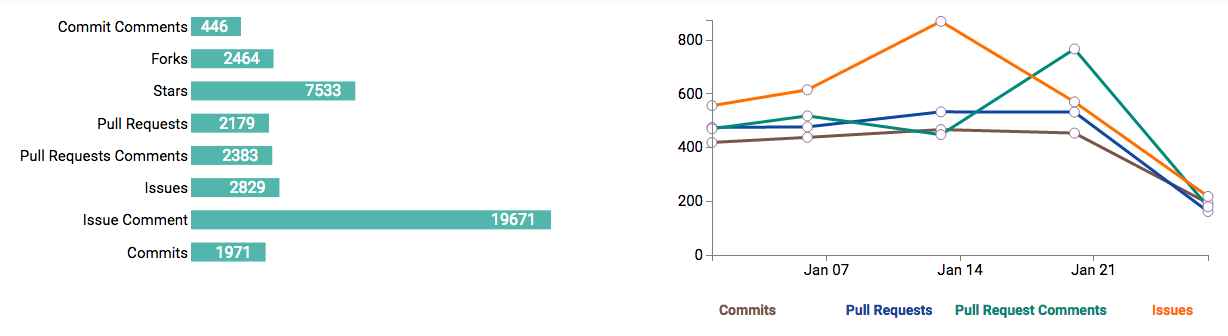
\includegraphics[height=4.5cm, width=17cm]{native}
\caption{React Native Data}
\end{figure}

While this is amazing in itself, we have only shown sum totals of data overall. This brings us to our last feature: the \textbf{monthly date picker}.

\subsection {Monthly Date Picker}

One of the most important aspects of any visualization is to be able to bring in dynamic data, allowing trends to be more discoverable and to help tell a more meaningful story. To do so, we have implemented a feature which allows the user to select which type of dataset they would like to view:

\begin {itemize}
	\item \textbf{Total}: The sum total of the last 4 month's worth of data.
	\item \textbf{Monthly}: The monthly totals of the selected month. Currently supports January, February, March and April.
\end {itemize}

By selecting to visualize a specific month of data, all of our visualizations will dynamically update themselves. This in itself is an extremely powerful feature of our visualization, and has many more implications which we discuss in section 5.1. With the implemented features discussed, we move into describing our technology stack.

\newpage

\section {How?}

Our first order of business was to gather the appropriate data. To do this, we took several approaches and collected our datasets together, as there was no single method which retrieved everything that we wanted. In this section we break down all of the decisions and technologies that helped us bring this project together.

\subsection {Github API}

Using the Github API, we are able to write scripts using both \textbf{node.js} and \textbf{python} which retrieved a list of all (public) Facebook repositories on Github. Among this data, we also collected various metadata such as:

\begin {itemize}
	\item Number of contributors
	\item Total number of commits
	\item Total number of issues
	\item Total number of stars
	\item Language of each repository
\end {itemize}

While this data was sufficient for some tasks, we were unable to drill down further. For instance, how would we determine how many stars, commits, or issue events occurred from day-to-day? Even if this was possible through the API, we ended up getting rate limited quite often due to the sheer number of requests we were sending out. However, we soon discovered a new means of data collection: \textbf{Github Archive}.

\subsection {Github Archive}

Github Archive\footnote{Github Archive: https://www.githubarchive.org/} keeps track of all events that occur across Github on a daily basis. In any given day, \textbf{json} files are generated which store every action taken by any user: \textbf{push events}, \textbf{issue comment events}, \textbf{issue assigned events}, etc. In fact, Github Archive allows us to drill down as deep as possible in order to aggregate all of the data on a daily basis. In order to process the data, several bash scripts were written which iteratively downloads the datasets from Github Archive on a daily basis for a given month. Once the data is retrieved, it is parsed using various \textbf{Python} scripts. We have scripts for processing both the total data over the last few months, as well as for totaling the data for any specific month. Moreover, we have scripts that process the datasets into the correct formats for the event bar chart, event time series and repository tree map. For some rough ideas regarding data size, each month of data which we parsed was upwards of 100+ GB.

\subsection {Data Driven Documents}

Lastly, we use \textbf{Data Driven Documents}\footnote{D3: https://d3js.org/} (D3) to create our visualizations. D3 is a powerful JavaScript library which allows developers to hand-craft their visualizations in any shape or form that they please (at the expense of code complexity). We built the tree map, bar chart and time series in parallel while fleshing out their interactions. Lastly, we implemented interactivity amongst all of the visualizations together.

\section {So What?}

After playing around with our visualization, we can answer various questions about \textbf{project lifespans}. As shown in earlier examples, we can easily deduce the lifespan of projects such as react-native, whose lifespan currently consists of massive bug fixes and feature additions by looking at the ratio of issue events versus pull requests and commits. Moreover, we can stumble upon more trends as shown in Figure 11.

\newpage

\begin{figure}[h!]
\centering
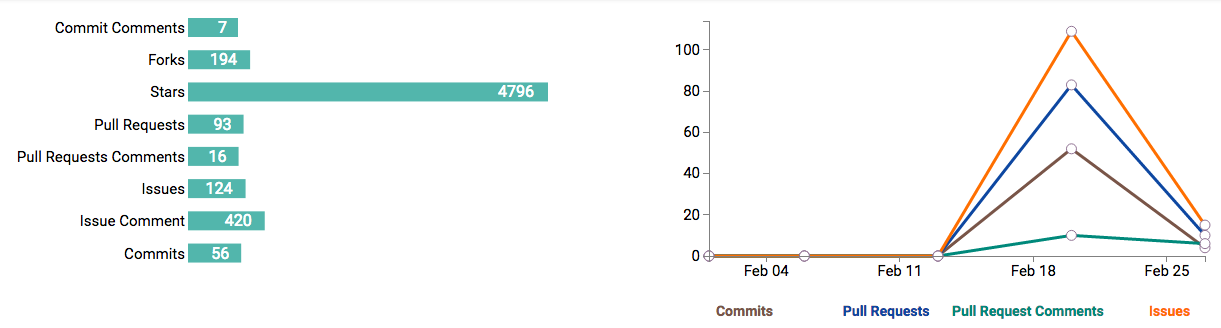
\includegraphics[height=4.5cm, width=17cm]{draft}
\caption{Visualizing Draft.js}
\end{figure}

Here we see a massive spike between the third and fourth week in the event time series. We can see an overwhelming number of issues, tons of pull requests and commits with few pull request comments. It turns out that this was the week that \textbf{draft.js} went public on Github:

\begin{figure}[h!]
\centering
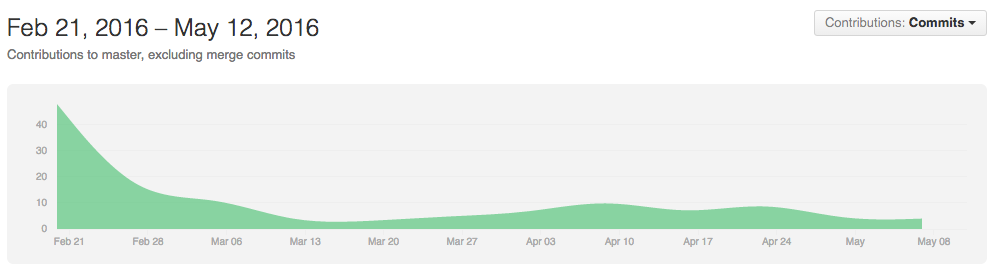
\includegraphics[height=4.5cm, width=17cm]{graph}
\caption{Github Contributor Graph for Draft.js}
\end{figure}

Even without knowing this, we can also speculate this from the overwhelming number of \textbf{star} events with respect to all other events. Typically, a repository which has gained a lot of traction on Github will receive an overwhelming number of stars which is evident here. To take it a step further, those who frequent Hacker News knows that stories which are top-voted and happen to be Github projects tend to skyrocket with stars. Unsurprisingly, within that same week there was a top trending Hacker News\footnote{Draft.js Hacker News Post: https://news.ycombinator.com/item?id=11153757} post regarding draft.js. Overall, our visualization does not essentially seek to answer questions, but aims to bring light to trends in Github data which are not immediately obvious. Moreover, we can quickly deduce that projects which occupy a smaller region in the tree map are projects which are either stagnant or were simply stand-alone libraries which were created to serve a single purpose such as CParser (Figure 13). 

\subsection {Future Work}

While projects such as Github [6] are extremely powerful, it is extremely limited by it's static dataset. By converting our project into a long-running web application, we can dramatically increase the potential of this project. We explore these ideas here.

\subsubsection {Specify User for Project Visualization}

Currently, our project is set to visualize all Facebook repositories on Github. However, it would be a great feature if we allowed the user to enter in any username on Github in order to visualize all of their repositories. This feature would allow the user to get insights in real-time for any user on Github, and could be a great asset to creating a weekly or monthly \textbf{digest} which users can subscribe to. Better yet, users may want to be able to specify a set of repositories or users and receive these visualizations in order to keep track of trending repositories.

\subsubsection {Custom Date Range Picker}

Currently, our date range picker only allows the user to visualize repositories across a given month or over the past few months in total. If we extended our application to use a date range picker which allowed the user to specify any date range, the flexibility and capabilities of this project would be extended greatly. Not only would this allow for more granularity in the visualization, it could even extend the project into a \textbf{productivity tracker} [5] and story lines [1].

\begin{figure}[t!]
\centering
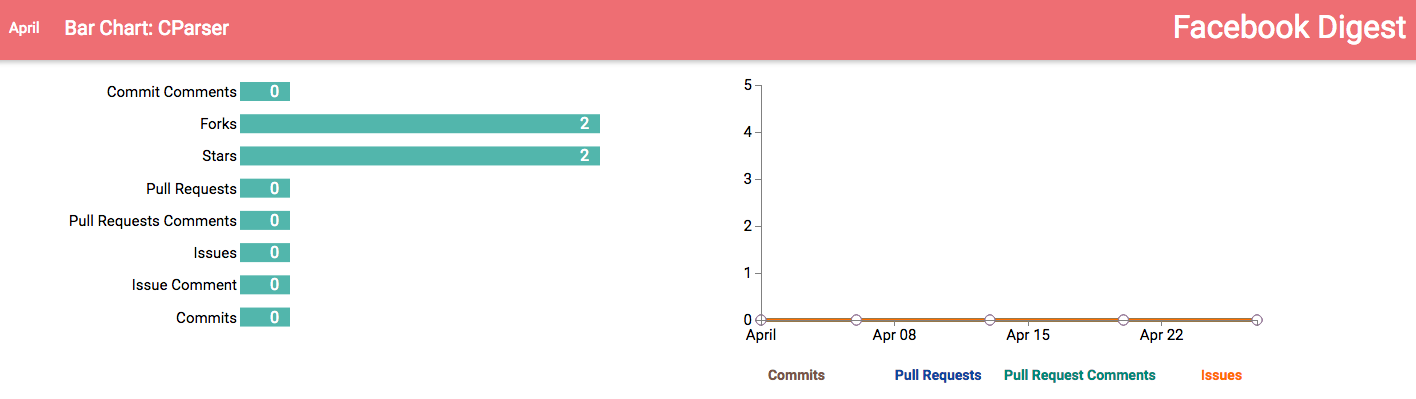
\includegraphics[height=4.5cm, width=17cm]{cparse}
\caption{Visualization for CParser}
\end{figure}

\section {Conclusion}

Visualizing open source code is one of the most challenging topics out there due to it's sheer complexity and generality. It is one of those ideas that is too general to determine which questions need to be answered, but rigid enough to come up with an endless amount of questions. In the beginning, we planned to build a tool which allows users to understand the lifespan of projects over the course of their inception. In the end, we developed a highly interactive tool which allows the user to understand trends for a group of repositories through various metrics and metadata. Our end goal is a web application which gives the user far more flexibility in terms of filters, date pickers and repository selections, allowing an infinite number of questions to be asked and answered. At the end of this project, we can more easily understand which projects out there are simply \emph{flash in the pan} projects - that is, projects which serve no long-term purpose. Moreover, we can analyze how successful projects such as \textbf{react.js} and \textbf{react-native} persevere - through commits, issues and so on. Overall, this project was amazing to work on and we certainly learned a lot in terms of creating a simple but powerful set of interactive visualizations. It was certainly run to work on, plan and iterate over, and we hope to extend it to be an open source tool which others may use to draw meaningful conclusions from.

\newpage

\begin{thebibliography}{9}
 
\bibitem{einstein} 
Michael Ogawa, and Kwan-Liu Ma
\textit{Software evolution storylines}.
Proceedings of the 5th international symposium on Software visualization. ACM, 2010.

\bibitem{einstein} 
Michael Ogawa.
\textit{Code Swarm}.
http://vis.cs.ucdavis.edu/~ogawa/codeswarm/

\bibitem{einstein} 
Andrew Caudwell.
\textit{Gource}.
https://github.com/acaudwell/Gource

\bibitem{einstein} 
Artem  Zubkov.
\textit{Github Visualizer}.
http://ghv.artzub.com/

\bibitem{einstein} 
Albert Chieu, David Leonard, Jorge Yau
\textit{Technetium-Bitbucket Productivity Tracker}.
http://technetium.herokuapp.com/

\bibitem{einstein} 
Carlo Zapponi
\textit{Githut: A small place to discover languages in Github}.
http://githut.info/, 2014

\end{thebibliography}

\end{document}
